\section{FeedApp Design}
\label{feedapp_design}

In this section, we dive into designing \textbf{FeedApp}, including everything from the full process, idea formulation and ideation to the final iteration of the application. We would like to keep it as a straight number section. Hence it would be split into two important heads: \textbf{Use Cases, Domain and Architecture}.

\subsection{Use Cases}

Here are some examples of the key features of \textbf{FeedApp}:

\begin{itemize}
    \item \textbf{Create Poll:} Users can create a new poll by entering a question and the options to vote for.\\
    \textit{Example:} A teacher uses a poll to get feedback on the most effective teaching methods.
    
    \item \textbf{Edit Poll:} Users can update the details of polls they have created, such as the question or voting options.\\
    \textit{Example:} A poll creator modifies the options of a poll to include a new choice.
    
    \item \textbf{Delete Poll:} Users can remove their own polls from the system, which also deletes associated votes.\\
    \textit{Example:} A user removes a poll once this is no longer valid since the end of the poll.
    
    \item \textbf{Vote on Poll:} Registered users can select a voting option in a poll.\\
    \textit{Example:} A student votes on the schedule of their preferred study group.
    
    \item \textbf{View Results:} Users can view aggregated poll results, either in real-time or after the poll closes.\\
    \textit{Example:} A user checks which option received the highest votes in a class poll.
    
    \item \textbf{Register and Log In:} New users can register for an account, and existing users can log in to access personalized features.\\
    \textit{Example:} A student logs into their account to participate in new polls.
    
    \item \textbf{Edit Vote:} Users can change their vote before the poll closes.\\
    \textit{Example:} A user initially selects "Option A" but later changes to "Option B" after reconsidering.
    
    \item \textbf{View Profile:} Users can review their activity, such as the polls they created and the votes they cast.\\
    \textit{Example:} A poll creator views the list of their active and closed polls.
    
    \item \textbf{Log Out:} Users can securely end their session.
\end{itemize}

The diagram below visually represents how users interact with \textbf{FeedApp}:

\begin{figure}[thb]
	\centering
	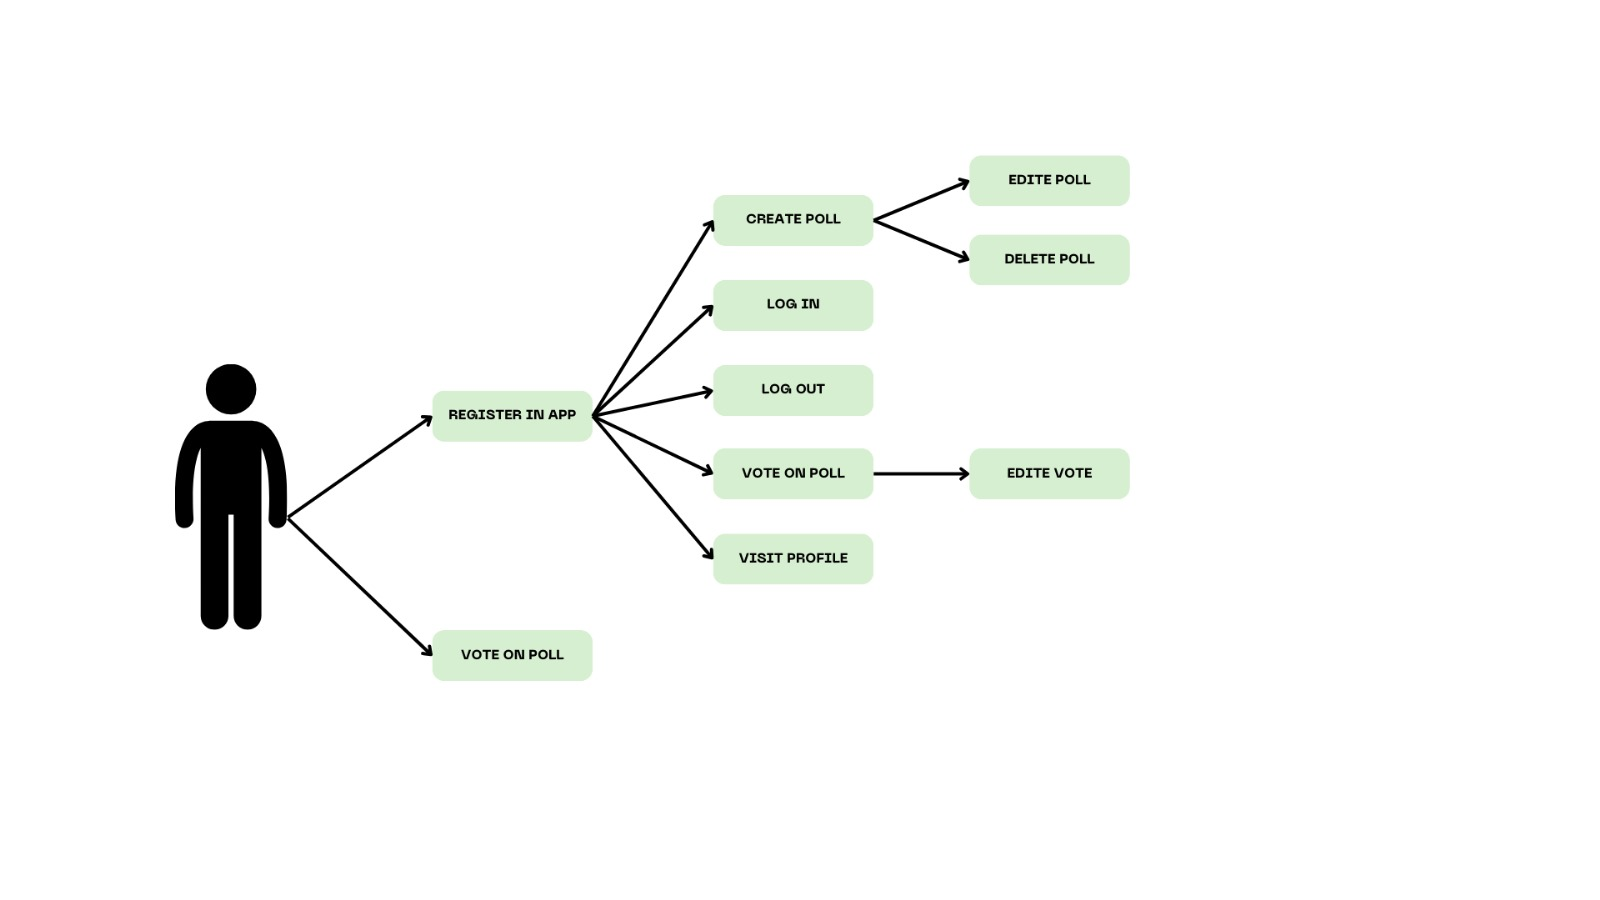
\includegraphics[scale=0.5]{figs/usecases.jpg}
	\caption{User interaction diagram for FeedApp.}
	\label{fig:feedapp_diagram}
\end{figure}


\subsection{Domain}

The \textbf{FeedApp} domain model underpins the business logic and data structure, defining the core entities and their relationships. This ensures a structured and scalable design.

\subsubsection{Key Entities}

\begin{enumerate}
    \item \textbf{User}
    \begin{itemize}
        \item \textbf{Relationships:}
        \begin{itemize}
            \item A user can create multiple polls.
            \item A user can participate in multiple votes.
        \end{itemize}
        \item \textbf{Description:} This class represents individuals interacting with the system as creators or participants in polls.
    \end{itemize}
    
    \item \textbf{Poll}
    \begin{itemize}
        \item \textbf{Attributes:}
        \begin{itemize}
            \item \texttt{id (Integer):} A unique identifier.
            \item \texttt{title (String):} The poll title.
            \item \texttt{question (String):} Refers to the poll question.
            \item \texttt{createdAt (Instant):} Creation timestamp.
            \item \texttt{validUntil (Instant):} Expiration timestamp.
            \item \texttt{user\_id (Integer):} Creator's identifier.
        \end{itemize}
        \item \textbf{Relationships:}
        \begin{itemize}
            \item The poll belongs just to one user.
            \item Can contain multiple vote options.
            \item Can have multiple associated votes.
        \end{itemize}
        \item \textbf{Description:} Is a central entity linking questions, options, and participants.
    \end{itemize}
    
    \item \textbf{VoteOption}
    \begin{itemize}
        \item \textbf{Attributes:}
        \begin{itemize}
            \item \texttt{id (Integer):} A unique identifier.
            \item \texttt{caption (String):} Option description.
            \item \texttt{presentationOrder (Integer):} Display order.
            \item \texttt{poll\_id (Integer):} Associated poll.
        \end{itemize}
        \item \textbf{Relationships:}
        \begin{itemize}
            \item Each VoteOption belongs to one poll.
            \item It’s linked to multiple votes.
        \end{itemize}
        \item \textbf{Description:} Represents all the choices available for users to select in a poll.
    \end{itemize}
\end{enumerate}


\subsubsection{Vote}

\begin{itemize}
    \item \textbf{Attributes:}
    \begin{itemize}
        \item \texttt{id (Integer):} A unique identifier.
        \item \texttt{votedAt (Instant):} Vote timestamp.
        \item \texttt{user\_id (Integer):} Voter's identifier.
        \item \texttt{voteOption\_id (Integer):} Selected option.
    \end{itemize}
    \item \textbf{Relationships:}
    \begin{itemize}
        \item Each vote is made by one user.
        \item Each vote is linked to one vote option.
    \end{itemize}
    \item \textbf{Description:} Captures voting activity, storing the user's choice in a poll.
\end{itemize}

\subsubsection{Key Relationships}

\begin{itemize}
    \item \textbf{User $\leftrightarrow$ Poll (1:N):} Each user can create multiple polls, but a poll belongs to one user.\\
    \textit{Example:} A teacher creates several polls for different courses.

    \item \textbf{Poll $\leftrightarrow$ VoteOption (1:N):} A poll can have multiple vote options, allowing users to provide various responses.\\
    \textit{Example:} A poll on favorite programming languages includes options like "Python," "Java," and "C++."

    \item \textbf{Poll $\leftrightarrow$ Vote (1:N):} A poll can receive multiple votes, reflecting participant responses.\\
    \textit{Example:} Students vote on their preferred class schedule.

    \item \textbf{VoteOption $\leftrightarrow$ Vote (1:N):} Each vote is tied to a specific option within a poll.
\end{itemize}

\subsubsection{UML Class Diagram}

\begin{figure}[h!]
    \centering
    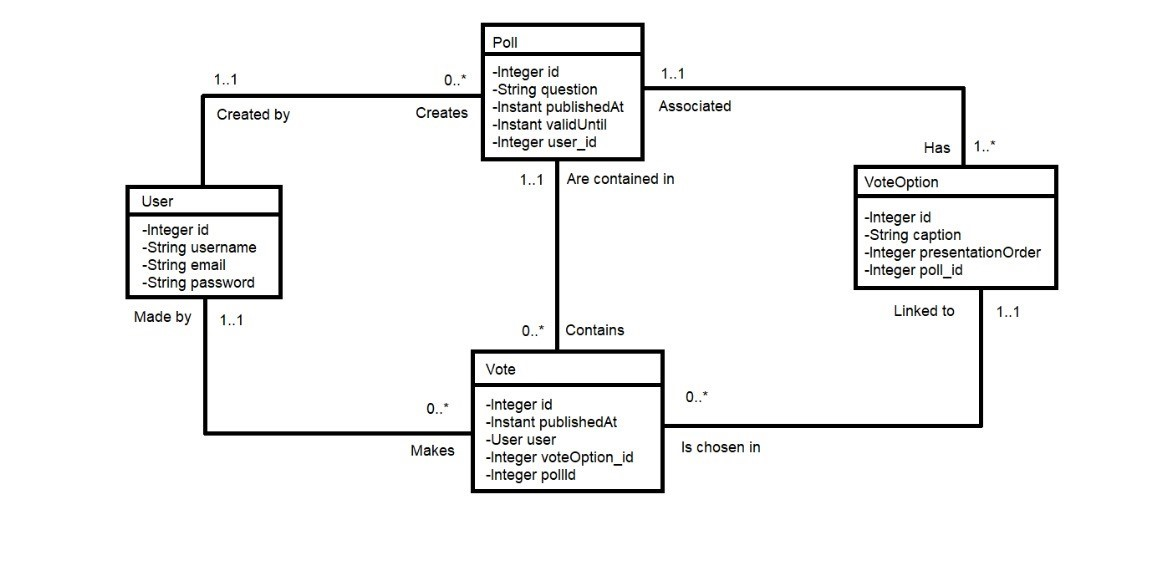
\includegraphics[width=0.9\textwidth]{figs/uml_diagram.jpg} 
    \caption{UML Class Diagram for FeedApp}
    \label{fig:uml_class_diagram}
\end{figure}

The UML diagram visualizes these relationships and cardinalities, ensuring that FeedApp's business logic is both intuitive and maintainable.


\subsection{Architecture}

This domain model was selected to ensure flexibility, scalability, and integrity.

\subsubsection{Choosing Technologies}

\begin{itemize}
    \item \textbf{Frontend:} JSP and CSS for interface creation and styling.
    \begin{itemize}
        \item \textbf{JSP (JavaServer Pages):} Technology for creating dynamic web pages by combining HTML and Java logic, enabling interactive interfaces.
        \item \textbf{CSS:} Style sheet language used to customize the appearance of web pages, enhancing the visual user experience.
        \item \textbf{JavaScript:} Programming language used to add interactive features like animations (confetti, loaders) and dynamic modals to improve user engagement.
    \end{itemize}

    \item \textbf{Backend:} Java servlets for business logic.
    \begin{itemize}
        \item \textbf{Java Servlets:} Java components that handle server-side requests, enabling backend logic for dynamic web applications.
    \end{itemize}

    \item \textbf{Database:} SQLite for structured data storage and MongoDB for dynamic data handling.
    \begin{itemize}
        \item \textbf{JDBC (Java Database Connectivity):} API for efficient interaction between Java applications and relational databases like SQLite.
        \item \textbf{SQLite:} An efficient relational database to organize your structured data with well-defined relationships employing primary and foreign keys.
        \item \textbf{MongoDB:} A NoSQL database commonly known for its use of Semi-Structured data, useful to store application statistics.
    \end{itemize}

    \item \textbf{Data Analysis \& Communication:} Real-time data integration and management with RabbitMQ.
    \begin{itemize}
        \item \textbf{RabbitMQ:} A messaging system that allows application components to communicate in real time and process asynchronously.
    \end{itemize}
\end{itemize}

\subsubsection{Development Highlights}

\begin{figure}[h!]
    \centering
    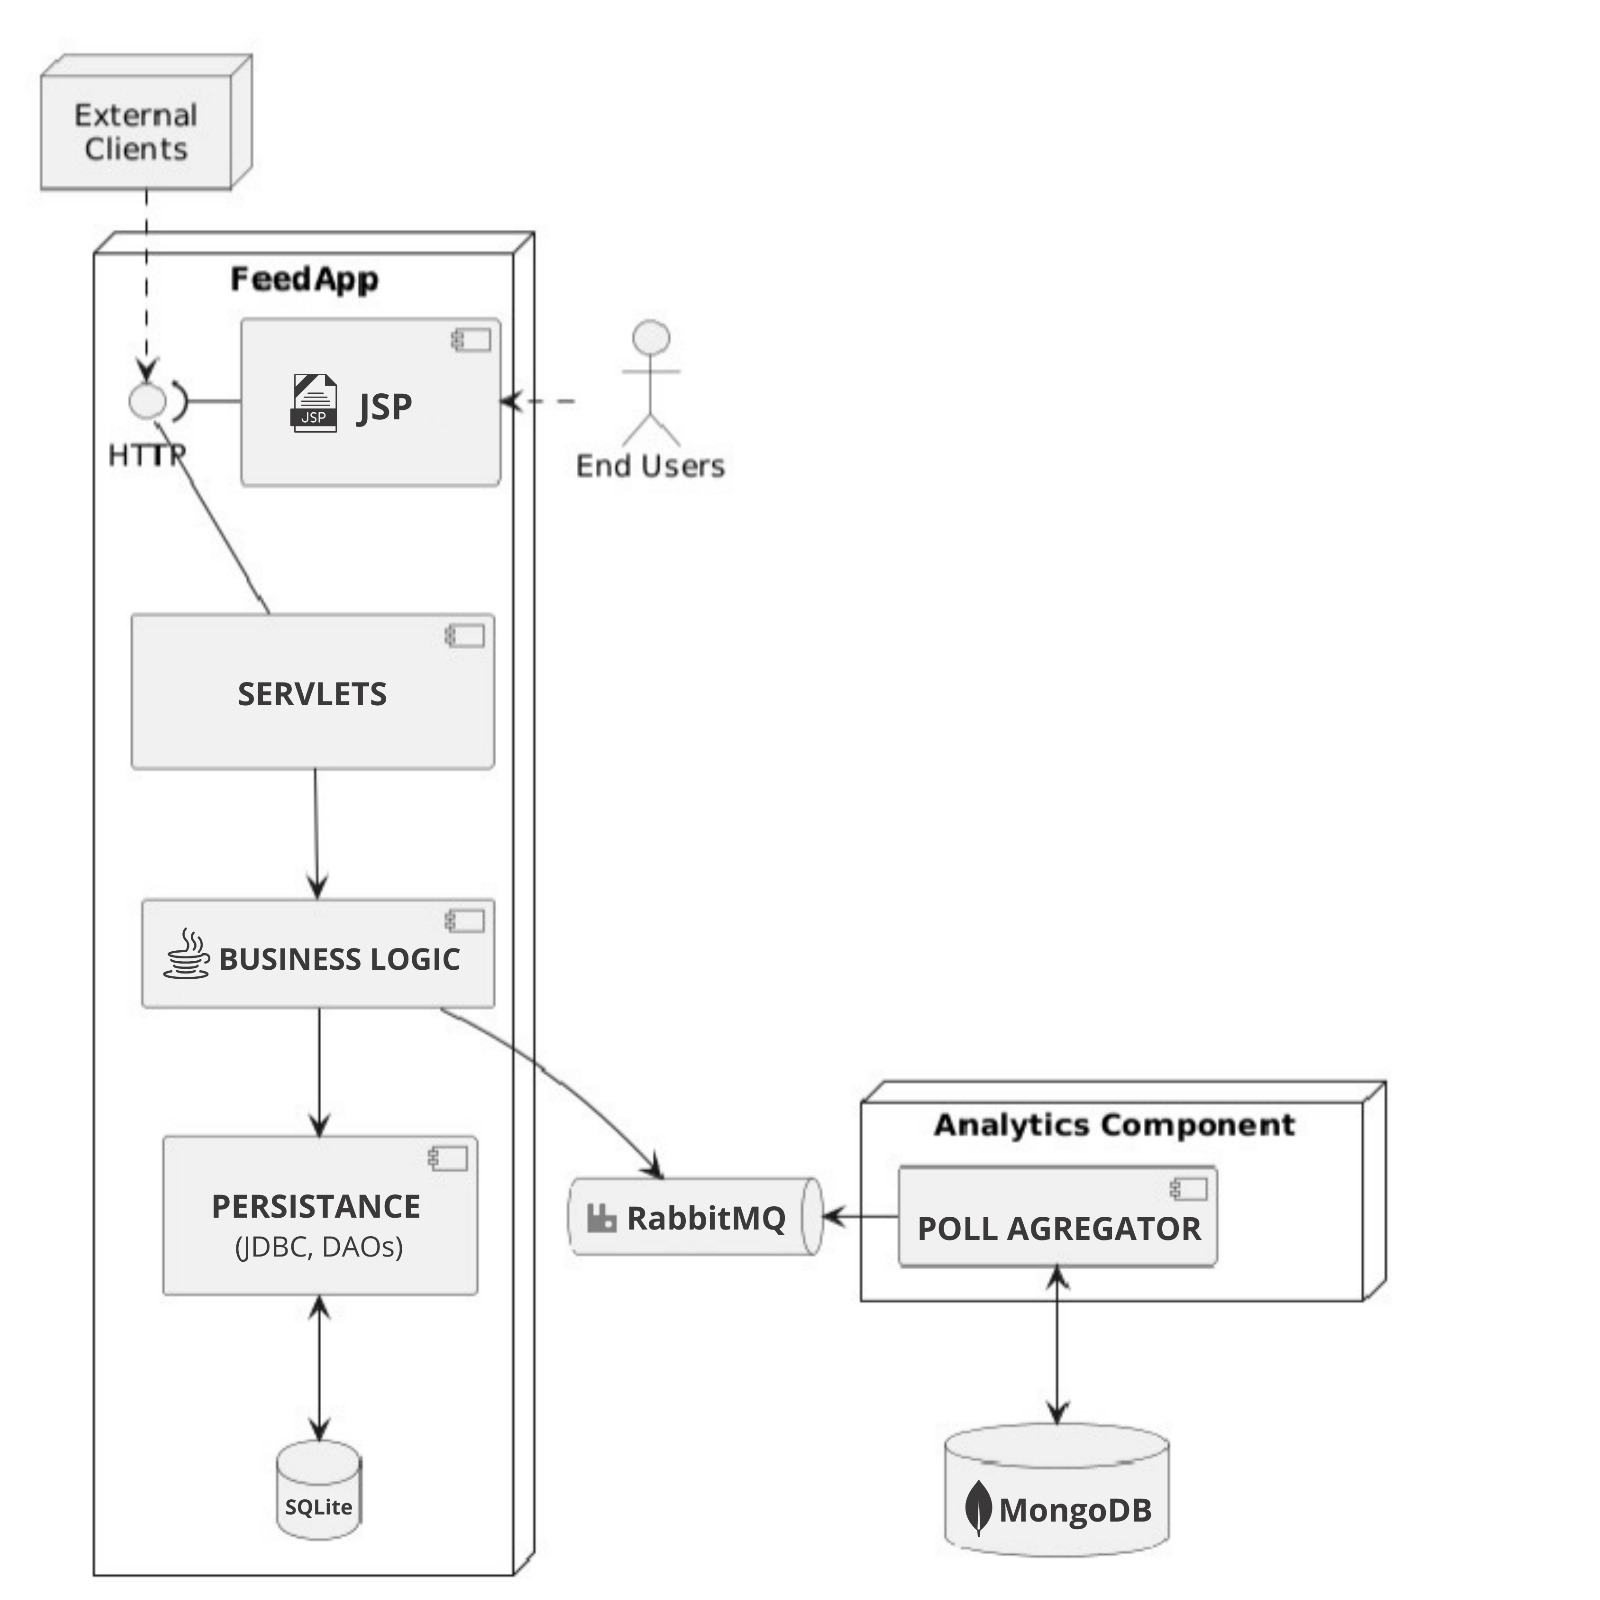
\includegraphics[width=0.9\textwidth]{figs/architecture_diagram.jpg} 
    \caption{Development Highlights Diagram for FeedApp}
    \label{fig:development_highlights}
\end{figure}

Here is the description of how each component communicates in the workflow:

\begin{enumerate}
    \item \textbf{External Clients:}
    \begin{itemize}
        \item End users interact with the application via HTTP requests, which are routed to the \textbf{FeedApp}.
    \end{itemize}

    \item \textbf{FeedApp:}
    \begin{itemize}
        \item \textbf{JSP:} Frontend layer. It receives user input (over HTTP) and creates dynamic web pages in return to the users. SERVLETS communicate directly with JSP.
        \item \textbf{SERVER SIDE COMPONENTS: SERVLETS:} It is a controller. It gets requests coming from the front end (JSP); it processes them and sends requests to the BUSINESS LOGIC layer.
        \item \textbf{BUSINESS LOGIC:} This is the application core. It handles the data obtained through SERVLETS and communicates with the PERSISTENCE layer to perform database-related actions.
        \item \textbf{PERSISTENCE:} Use of JDBC and DAOs to perform CRUD (Create, Read, Update, Delete) operations on the \textbf{SQLite} database.
    \end{itemize}

    \item \textbf{SQLite:}
    \begin{itemize}
        \item Serves as the primary database, storing structured data such as user information, polls, and votes. It is accessed through the PERSISTENCE layer.
    \end{itemize}

    \item \textbf{RabbitMQ:}
    \begin{itemize}
        \item Acts as a message broker between the \textbf{FeedApp} and the \textbf{Analytics Component}.
        \item After critical events (e.g., poll creation or vote submission), BUSINESS LOGIC publishes messages to RabbitMQ to update analytics asynchronously.
    \end{itemize}

    \item \textbf{Analytics Component:}
    \begin{itemize}
        \item The \textbf{Poll Aggregator} receives messages from RabbitMQ and updates the statistics in \textbf{MongoDB}, which stores semi-structured data like user counts, polls created, and votes recorded.
    \end{itemize}

    \item \textbf{MongoDB:}
    \begin{itemize}
        \item A NoSQL database that holds analytics and semi-structured data enabling the system to manage large-scale and dynamic data efficiently.
    \end{itemize}
\end{enumerate}